\documentclass{report}

\usepackage{textcomp}
\usepackage{graphicx}
\usepackage{fancyhdr}
\usepackage{subcaption}
\usepackage{multicol}
\usepackage{outlines}
\usepackage{minted}
%===================================
\newcommand{\classinfo}{{\bf RHEL 134 \\ Week 02 Labs}\\{\it CIT 218}\\{Chaz Davis}}
\newcommand{\semester}{BCTC \\ Spring 2020}
%===================================
\newcommand{\mysection}[1]{\section*{#1}}
\newcommand{\mysubsection}[2]{\textbf{\romannumeral #1) #2}}
%===================================
\setlength{\headheight}{15.2pt}
\pagestyle{fancy}
\fancyhf{}
\lhead{ \fancyplain{}{Chaz Davis} }
\rhead{ \fancyplain{}{\today} }
\cfoot{ \fancyplain{}{\thepage} }
\renewcommand{\headrulewidth}{0.5pt}
\renewcommand{\footrulewidth}{0pt}

%===================================
\title{\classinfo}
\author{\semester}
\date{\today}

%===================================

\begin{document}

\maketitle

%===================================
\mysection{Questions}

\mysubsection{1}{Echo the hostname of the system to a file in the /tmp
directory in 5 minutes using the at command. List the scheduled at job.
Provide the output.}\\
I Ran the Commands:
{\scriptsize{\verb$echo "hostname > /tmp/hostname" | at now +5min$}\normalsize}
to set up the job. I then ran {\scriptsize{\verb$atq$}\normalsize} to show the
job saved into the queue. You can see in Fig.~\ref{Week2}\subref{Week2Q1} 
on Pg.~\pageref{Week2}.


\noindent\mysubsection{2}{Create a cronjob that echoes your first and last name
every Sunday at 2pm during the month of March. Provide the details.}\\
I ran {\scriptsize{\verb$crontab -e$}\normalsize} to get into the cronjob
setup. Once there I created a new cronjob:


\begin{minted}
[
frame=lines,
framesep=2mm,
baselinestretch=1.2,
fontsize=\footnotesize,
linenos
]
{vim}
  0 14 * 3 0 echo "Chaz Davis" >> /home/student/My_Name_Cron_Job
\end{minted}

\begin{itemize}
  \item{Where {\scriptsize{\verb$0 14$}\normalsize} stands for 1400 or 2pm.} 
  \item{Where {\scriptsize{\verb$* 3 0$}\normalsize} stands for every sunday in
    march} 
  \item{Finally, {\scriptsize{\verb$echo "Chaz Davis"$}\normalsize} is sending
    my name into a particular file} 
\end{itemize}


For the screenshot of the terminal see
Fig.~\ref{Week2}\subref{Week2Q2} 
on Pg.~\pageref{Week2}.

\noindent\mysubsection{3}{Provide the output of all nice levels for current
running processes with the highest nice levels sorted at the top.}\\
From the commandline I ran:
{\scriptsize{\verb$ps axo pid,comm,nice,cls --sort=nice$}\normalsize}, so that
I could get the processes with {\scriptsize{\verb$ps$}\normalsize}, where 
{\scriptsize{\verb$axo$}\normalsize}, the `ax' means show all running
processes, and the `o' means format the output. In this case I wanted the
format to contain {\scriptsize{\verb$pid,comm,nice,cls$}\normalsize}, or
process id, command, nice level, and class. Finally, the 
{\scriptsize{\verb$--sort=nice$}\normalsize} means that we will sort by the
nice column. See Fig.~\ref{Week2}\subref{Week2Q3} 
on Pg.~\pageref{Week2}.


\noindent\mysubsection{4}{Run the top command in the background. Change the nice
level of the backgrounded top process to the lowest priority. Provide
the output.}\\
I first ran the command {\scriptsize{\verb$top &$}\normalsize} to start top and
place it into the background. I then ran {\scriptsize{\verb$ps$}\normalsize}
just to show the running processes. I then used its PID `3810' to run the
command {\scriptsize{\verb$sudo renice -n -20 3810$}\normalsize}, which takes
the nice value of top from 0 to -20, or the lowest nice value. You can see the
total output and screenshots in Fig.~\ref{Week2}\subref{Week2Q4} 
on Pg.~\pageref{Week2}.


\begin{figure}[!hbt]\centering
  \subfloat[Echoing Hostname into /tmp file]{\label{Week2Q1}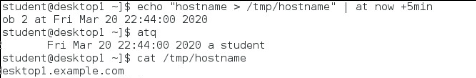
\includegraphics[width=.70\linewidth]{Figures/2020-03-20-225236_476x78_scrot.png}}\par
\subfloat[Echoing my name into crontab]{\label{Week2Q2}
\includegraphics[width=.60\linewidth]{Figures/2020-03-20-231322_593x137_scrot.png}}\par
\subfloat[Processes sorted by nice]{\label{Week2Q3}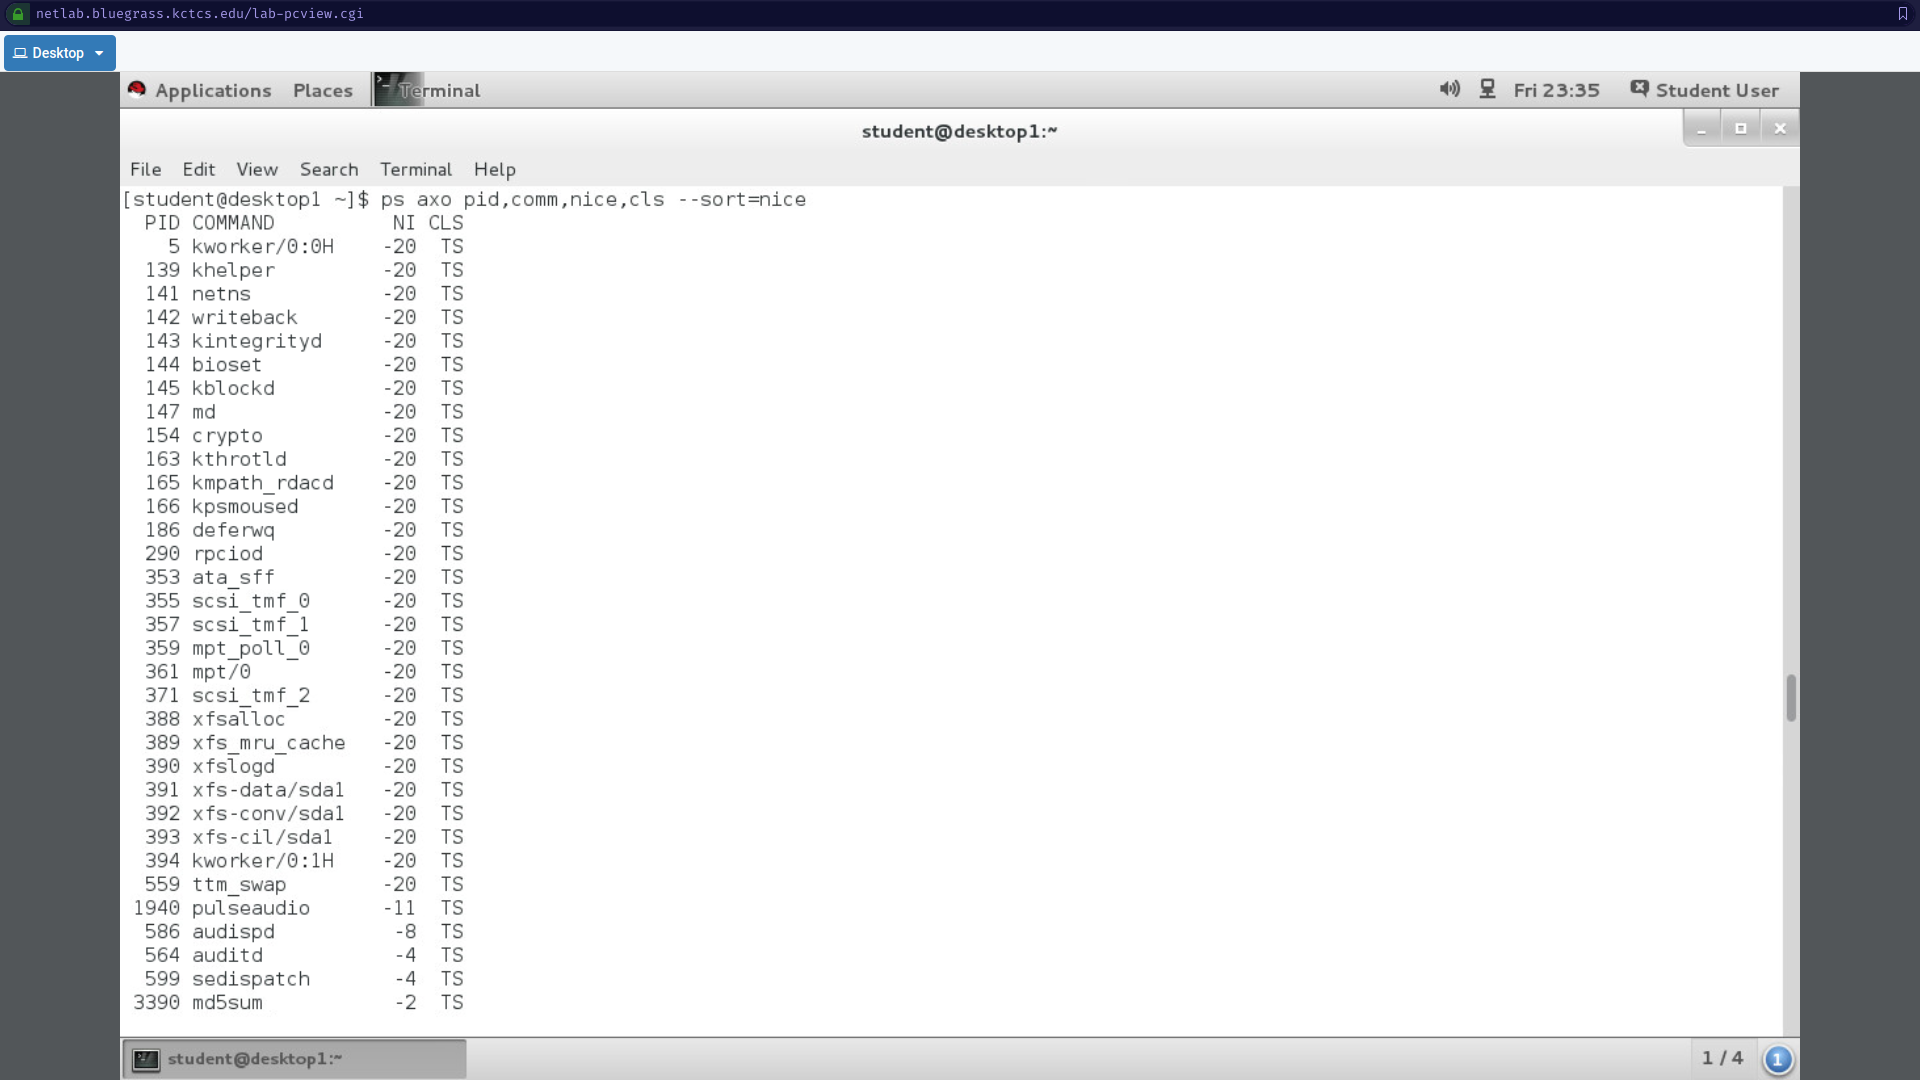
\includegraphics[width=.90\linewidth]{Figures/2020-03-20-233559_1920x1080_scrot.png}}\par
\subfloat[Changing the nice level of top]{\label{Week2Q4}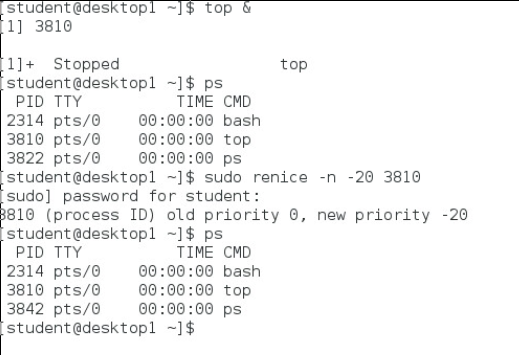
\includegraphics[width=.65\linewidth]{Figures/2020-03-20-235647_519x355_scrot.png}}\par
\caption{Week 2 Screenshots}\label{Week2}
\end{figure}



%===================================
\end{document}
